\documentclass{article}

\usepackage[fleqn]{amsmath}
\usepackage{amssymb}
\usepackage{hyperref}
\usepackage{url}
\usepackage{graphicx}
\usepackage{geometry}
\usepackage{babel}
\usepackage{enumitem}
\usepackage{parskip}
\usepackage{chemfig}
\usepackage{pdfpages}
\usepackage{tikz}
\usepackage{fancybox}
\usepackage{makecell}
\usepackage{pgfplots}
\usepackage{soul}
\usepackage{ulem}
\usepackage{wrapfig}
\usepackage{subcaption}
\usepackage[T1]{fontenc}
\usepackage{esvect}
\usepackage{xcolor}
\usetikzlibrary{arrows}
\usetikzlibrary{decorations.pathreplacing}
\pgfplotsset{compat=1.17}

\geometry{
    a4paper,
    total={170mm, 257mm},
    left=20mm,
    top=20mm
}

\hypersetup{
    colorlinks=true,
    linkcolor=black,
    urlcolor=blue,
    pdftitle={Context 1}
}

\newcommand{\figbox}[1]{ 
    \begin{figure*}[ht!]        
        \begin{center}            
            \fbox{#1}        
        \end{center}    
    \end{figure*}
}

\newcommand{\wrapfill}{
    \par
    \ifnum \value{WF@wrappedlines} > 0
        \addtocounter{WF@wrappedlines}{-1}%
        \null\vspace{
            \arabic{WF@wrappedlines}
            \baselineskip
        }
        \WFclear
    \fi
    \phantom{}
}

\newcommand{\cfig}[1]{%
  \begin{figure*}[ht!]%
    \centering%
    #1%
  \end{figure*}%
}

\newcommand{\difference}{\,\backslash\,}
\newcommand{\rem}{\underline{Remark}: }
\newcommand{\nots}{\underline{Notation}: }
\newcommand{\prf}{\underline{Proof}: }
\newcommand{\exs}{\underline{Example}: }
\newcommand{\defs}{\underline{Definition}: }
\newcommand{\wrn}{\underline{Warning}: }
\newcommand{\sht}{\ |\ }


% === TEXT ===
\title{\textbf{User scenario - Context 1\\ HSLU, Semester 1}}
\author{Matteo Frongillo}

\begin{document}

% Titolo e logo
\begin{titlepage}
    \centering
    \vspace*{1cm}
    
    {\Huge \textbf{User Scenario}}\\[1.5cm]
    
    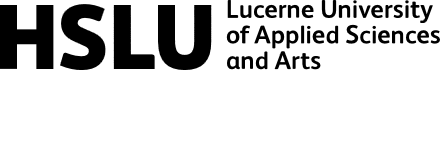
\includegraphics[width=0.4\textwidth]{media/hslu-svg-logo.png}\\[2cm] % Sostituisci LOGO con il percorso dell'immagine
    
    \vspace{1.5cm}
    \large
    \textbf{University Name}\\[1cm]
    \textbf{Your Name}\\
    \vfill
    \today
    
\end{titlepage}

\newpage
\tableofcontents

\newpage
% Contenuto
\section{User Scenario}
Il seguente scenario utente descrive la funzionalità del nuovo prodotto dal punto di vista dell'utente e risponde alle seguenti domande:

\begin{itemize}
    \item Quale problema viene risolto con il prodotto o quale bisogno viene soddisfatto?
    \item Chi utilizzerà il prodotto?
    \item Come verrà utilizzata la funzionalità?
\end{itemize}

\section{Esempio: CampBrew}

\subsection{Problema}
Gli appassionati di campeggio e viaggiatori non possono godere di caffè di alta qualità dalle loro macchine da caffè a capsule, poiché le macchine da caffè a capsule disponibili in commercio richiedono elettricità e sono troppo grandi e pesanti.

\subsection{Obiettivo}
Una macchina da caffè a capsule che sia compatta, portatile e funzioni senza la necessità di una presa elettrica.

\subsection{Descrizione del prodotto}
La macchina da caffè CampBrew dovrebbe essere un'evoluzione delle macchine da caffè a capsule disponibili in commercio, integrando la qualità e la funzionalità di una macchina a capsule standard in un formato più piccolo e leggero, facile da trasportare in uno zaino. Inoltre, l'involucro dovrebbe essere robusto e stabile per soddisfare i requisiti del campeggio. La macchina dovrebbe avere una fonte di alimentazione indipendente, permettendo agli utenti di gustare un caffè di alta qualità ovunque e in qualsiasi momento.

\subsection{Target}
La macchina da caffè CampBrew è ideale per coloro che non vogliono rinunciare al caffè di alta qualità durante i viaggi o il campeggio.





\end{document}